\documentclass{standalone}
\usepackage{tikz}
\usetikzlibrary{angles, quotes} % for angle marks

\begin{document}
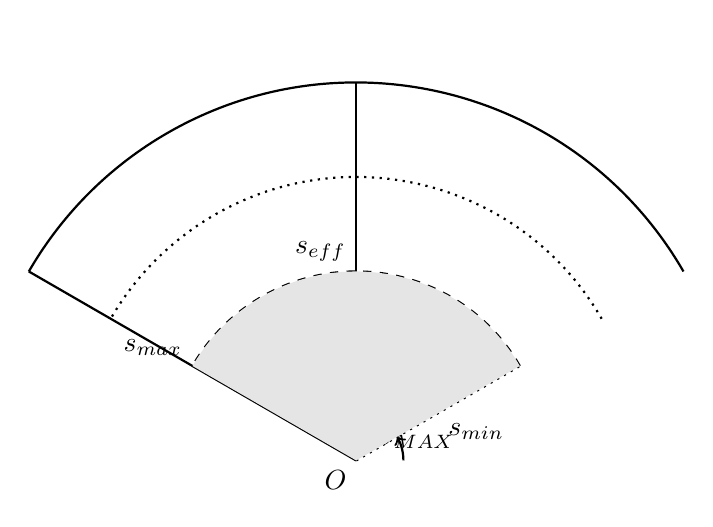
\begin{tikzpicture}[scale=1.2]

% Define coordinates
\coordinate (O) at (0,0);
\coordinate (A) at (90:4);   % Radius for s_eff
\coordinate (B) at (30:2);   % Radius for s_min
\coordinate (C) at (150:4);  % Radius for s_max

% Draw circles/arcs
\draw [thick] (30:2) arc (30:150:2) [dashed]; % Inner dashed arc
\draw [thick] (30:3) arc (30:150:3) [dotted]; % Middle dotted arc
\draw [thick] (30:4) arc (30:150:4);          % Outer solid arc

% Draw radii
\draw [thick] (O) -- (A) node[midway, above left] {$s_\text{eff}$};
\draw [thick, dotted] (O) -- (B) node[midway, below right] {$s_\text{min}$};
\draw [thick] (O) -- (C) node[midway, above left] {$s_\text{max}$};

% Label origin
\node[below left] at (O) {$O$};

% Draw angle
\draw[thick, ->] (0.5,0) arc [start angle=0, end angle=30, radius=0.5];
\node at (0.65,0.25) {$\theta_{\text{MAX}}$};

% Background fill
\fill[gray!20] (30:2) arc (30:150:2) -- (O) -- cycle;

\end{tikzpicture}
\end{document}